\section{Language theory}

\subsection{Expressions and statements}

A statement is a complete line of code that performs some action. 
An expression is any section of code that evaluates to a value.

General rule of thumb: if you can print it or assign it to a variable, it's an expression. If you can't, it's a statement. 

Examples of expressions: 
\begin{lstlisting}
2 + 2
3 * 7
1 + 2 + 3 * (8 ** 9) - sqrt(4.0)
min(2, 22)
max(3, 94)
round(81.5)
"foo"
"bar"
"foo" + "bar"
None
True
False
2
3
4.0
\end{lstlisting}

Examples of statements: 
\begin{lstlisting}
if CONDITION:
elif CONDITION:
else:
for VARIABLE in SEQUENCE:
while CONDITION:
try:
except EXCEPTION as e:
class MYCLASS:
def MYFUNCTION():
return SOMETHING
raise SOMETHING
with SOMETHING:
\end{lstlisting}
All of the above statements are syntax, but non of them does have a value. You cannot do \inlinecode{x = if CONDITION:}.


\subsection{Abstract syntax tree}
A \emph{tokenizer} parses a raw sourcefile and extracts from it an \emph{abstract syntax tree} (AST), which is a machine readable representation of the sourcecode (acutally, it's rather the other way round: the sourcecode is just the flat, human readable representation of the AST).

Consider the following js code: 

\begin{lstlisting}
var a = 3;
a + 5
\end{lstlisting}

This will be parsed into an AST like this: 

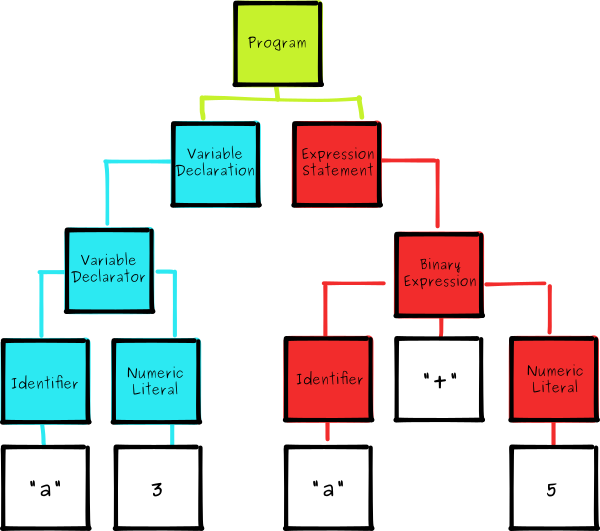
\includegraphics[width=0.4\textwidth]{images/ast.png}

